\documentclass[conference]{IEEEtran}
\usepackage{cite}
\usepackage{amsmath,amssymb,amsfonts}
\usepackage{algorithmic}
\usepackage{graphicx}
\usepackage{textcomp}
\usepackage{xcolor}
\usepackage{booktabs}
\usepackage{tikz}
\usetikzlibrary{shapes.geometric, arrows.meta, positioning, calc}

\begin{document}

\title{Deep Learning Based Detection of Adrenocortical Carcinoma and Ki-67 Growth Prediction from CT Images}

\author{
    \IEEEauthorblockN{Sakshi B. S.$^1$, Shwetha B. J.$^1$, Inchara N.$^1$, and Bhavana C. K.$^2$}
    \IEEEauthorblockA{$^1$UG Scholars, Department of Computer Science and Engineering\\
    $^2$Assistant Professor, Department of Computer Science and Engineering\\
    Maharaja Institute of Technology Thandavapura (MIT Thandavapura)\\
    Mysore -- Ooty Road, Just off NH 766, Nanjangud Taluk, Thandavapura, Karnataka, India\\
    Email: \{sakshibs, shwethabj, incharan\}@mitthandavapura.edu.in, bhavanack@mitthandavapura.edu.in}
}

\maketitle

\begin{abstract}
Adrenocortical Carcinoma (ACC) is an aggressive endocrine malignancy requiring timely identification and surgical resection. Contrast-enhanced Computed Tomography (CT) serves as the primary preoperative imaging tool; however, manual slice-by-slice tumor contouring across volumetric series is labor-intensive and subject to inter-reader disagreement. This paper presents an automated clinical decision support pipeline integrating a 3-layer CT integrity verification module, a tumor-focused 2D U-Net convolutional neural network, and quantitative morphometric profiling. Using the National Cancer Institute's public TCIA Adrenal-ACC-Ki67-Seg cohort of 53 patients (18,255 CT slices), a strict patient-level split (37 training, 7 validation, and 9 test subjects) was enforced to eliminate data leakage. Evaluated on 295 unseen test CT slices, the proposed network yielded an image-level tumor detection sensitivity of 92.55\%, precision of 89.39\%, F1-score of 90.94\%, and overall accuracy of 84.07\% at a decision threshold of 0.80. Across segmented tumor-positive slices, the network recorded a mean Dice similarity coefficient of 57.31\% and an Intersection over Union (IoU) of 50.74\%, reaching a peak single-slice Dice score of 95.94\%. The framework automatically extracts physical cross-sectional areas, craniocaudal volumetric burden, bounding diameters, and spatial proliferation indices, providing surgeons with reproducible quantitative measurements and automated report generation.
\end{abstract}

\begin{IEEEkeywords}
Adrenocortical Carcinoma (ACC), Deep Learning, U-Net, Medical Image Segmentation, Computed Tomography (CT), Ki-67 Proliferation, Morphometric Profiling, Clinical Decision Support.
\end{IEEEkeywords}

\section{Introduction}
Adrenocortical Carcinoma (ACC) represents an uncommon yet biologically virulent tumor arising from the adrenal cortex, presenting an annual incidence of 0.5 to 2.0 cases per million individuals \cite{moawad2023, fassnacht2018}. Surgical resection with clear margins (R0) offers the only realistic prospect of long-term cure. Multi-detector Computed Tomography (CT) provides essential anatomical detail of the retroperitoneal space, allowing clinicians to evaluate primary tumor dimensions, adjacent organ infiltration, and venous thrombus invasion into the inferior vena cava.

Despite modern imaging capabilities, objective radiographic evaluation of ACC presents major operational difficulties:
\begin{enumerate}
    \item \textit{Manual Delineation Overhead:} Abdominal CT studies routinely comprise 60 to 150 axial slices per patient. Tracing irregular, necrotizing tumor margins across sequential cross-sections demands substantial radiologist hours during acute oncologic admissions.
    \item \textit{Inter-Observer Discordance:} Low attenuation gradients between viable tumor tissue, central necrosis, and adjacent renal or hepatic parenchyma frequently lead to conflicting boundary definitions among reading clinicians.
    \item \textit{Limited Spatial Burden Profiling:} Routine radiological reporting relies on unidimensional RECIST measurements. Such static metrics fail to capture the longitudinal cross-sectional distribution and continuous volumetric burden necessary for complex operative planning.
\end{enumerate}

Convolutional neural networks, particularly symmetric encoder-decoder topologies such as U-Net \cite{ronneberger2015}, have shown high fidelity across medical segmentation benchmarks. Most existing studies address hepatic, renal, or pulmonary neoplasms, while adrenal lesions remain underexplored due to case rarity.

This work implements an automated clinical workflow addressing these gaps. The system incorporates an initial 3-layer input verification filter to reject non-CT uploads, a 1.95-million-parameter U-Net for binary tumor segmentation, automated physical morphometry calculation, and an interactive browser dashboard generating printable diagnostic summaries.

\section{Related Work}
Early abdominal CT segmentation algorithms relied on intensity thresholding, region growing, and parametric deformable active contours. While computationally light, these approaches struggle in high-grade ACC cases characterized by internal hemorrhagic necrosis, calcifications, and ill-defined boundaries against surrounding soft tissues.

The introduction of U-Net by Ronneberger et al. \cite{ronneberger2015} established a robust baseline for biomedical segmentation by concatenating fine-grained shallow encoder features with deep semantic decoder representations via skip connections. Subsequent challenges, notably KiTS19 for renal masses \cite{heller2021} and LiTS for liver neoplasms \cite{bilic2023}, highlighted the value of deep convolutional representations in the abdomen.

In adrenal imaging, prior computational studies predominantly investigated organ localization through multi-organ probabilistic atlases \cite{gibson2018} or differentiated benign adenomas from non-adenomas using non-contrast Hounsfield Unit (HU) attenuation wash-out values. In 2023, Moawad et al. published the Adrenal-ACC-Ki67-Seg cohort through The Cancer Imaging Archive (TCIA) \cite{moawad2023}, providing the first pathology-grounded voxel segmentations for ACC with matched Ki-67 proliferative indices. This study builds on that open resource to establish an end-to-end detection, segmentation, and morphometric profiling framework.

\section{Materials and Dataset}

\subsection{TCIA Adrenal-ACC-Ki67-Seg Cohort}
Experiments were conducted on the public Adrenal-ACC-Ki67-Seg dataset hosted by TCIA \cite{moawad2023}. The collection contains contrast-enhanced abdominal CT series from 53 patients with pathologically confirmed ACC, totaling 18,255 DICOM CT images. Ground-truth voxel segmentations were delineated by experienced abdominal radiologists and archived as standardized DICOM Segmentation (SEG) objects.

\subsection{Spatial Reconstruction and Registration}
Using \texttt{pydicom} and \texttt{nibabel}, each patient's DICOM SEG metadata was decoded to extract the referenced SOP Instance UIDs. The corresponding raw CT slices were spatially sorted along the craniocaudal axis according to their spatial image position attributes, constructing calibrated 3D NIfTI volumes. Spatial coordinate alignment, origin vectors, and affine matrices between reconstructed CT volumes and extracted binary tumor masks were verified across all 53 subjects.

\subsection{Patient-Level Data Partitioning}
To prevent data leakage, dataset partitioning was conducted strictly at the patient level rather than by random slice shuffling:
\begin{itemize}
    \item \textbf{Training Set:} 37 patients (1,622 slices: 1,473 tumor-positive, 149 background).
    \item \textbf{Validation Set:} 7 patients (178 slices: 150 tumor-positive, 28 background).
    \item \textbf{Held-Out Test Set:} 9 patients (295 slices: 255 tumor-positive, 40 background).
\end{itemize}
Slices from the 9 test patients remained completely withheld from network optimization and threshold tuning.

\subsection{CT Preprocessing and Windowing}
Raw CT attenuation values span $-1024$ to $+3071$ HU. An abdominal soft-tissue window was applied to suppress high-attenuation cortical bone while expanding retroperitoneal soft-tissue contrast:
\begin{equation}
    \text{Window Center (WL)} = +40\text{ HU}, \quad \text{Window Width (WW)} = 400\text{ HU}
\end{equation}
resulting in an effective intensity range of $[-160\text{ HU}, +240\text{ HU}]$. Attenuation values were clamped and linearly normalized to $[0.0, 1.0]$:
\begin{equation}
    I_{\text{norm}}(x,y) = \text{clip}\left(\frac{I(x,y) - (-160)}{400}, 0.0, 1.0\right)
\end{equation}
and standardized to a spatial resolution of $512 \times 512 \times 1$.

% --- ARCHITECTURE BLOCK DIAGRAM (TIKZ) ---
\begin{figure*}[!t]
\centering
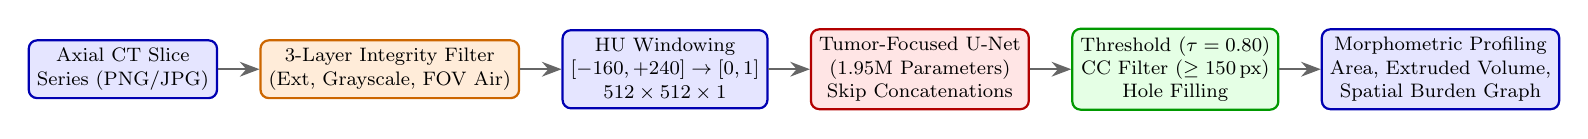
\begin{tikzpicture}[
    scale=0.88, every node/.style={transform shape},
    box/.style={rectangle, draw=blue!70!black, fill=blue!10, rounded corners=3pt, thick, align=center, font=\footnotesize, minimum height=0.75cm},
    filter/.style={rectangle, draw=orange!80!black, fill=orange!15, rounded corners=3pt, thick, align=center, font=\footnotesize, minimum height=0.75cm},
    unet/.style={rectangle, draw=red!70!black, fill=red!10, rounded corners=3pt, thick, align=center, font=\footnotesize, minimum height=0.75cm},
    post/.style={rectangle, draw=green!60!black, fill=green!10, rounded corners=3pt, thick, align=center, font=\footnotesize, minimum height=0.75cm},
    arrow/.style={-{Stealth[length=2.5mm]}, thick, draw=gray!80!black}
]
    % Pipeline Nodes
    \node[box] (input) at (0,0) {Axial CT Slice\\Series (PNG/JPG)};
    \node[filter, right=0.6cm of input] (val) {3-Layer Integrity Filter\\(Ext, Grayscale, FOV Air)};
    \node[box, right=0.6cm of val] (norm) {HU Windowing\\$[-160, +240] \to [0, 1]$\\$512 \times 512 \times 1$};
    \node[unet, right=0.6cm of norm] (unet) {Tumor-Focused U-Net\\(1.95M Parameters)\\Skip Concatenations};
    \node[post, right=0.6cm of unet] (thresh) {Threshold ($\tau=0.80$)\\CC Filter ($\ge 150$\,px)\\Hole Filling};
    \node[box, right=0.6cm of thresh] (out) {Morphometric Profiling\\Area, Extruded Volume,\\Spatial Burden Graph};

    % Connecting Arrows
    \draw[arrow] (input) -- (val);
    \draw[arrow] (val) -- (norm);
    \draw[arrow] (norm) -- (unet);
    \draw[arrow] (unet) -- (thresh);
    \draw[arrow] (thresh) -- (out);
\end{tikzpicture}
\caption{End-to-end diagnostic workflow: 3-layer image verification, U-Net segmentation, post-processing, and morphometric index calculation.}
\label{fig:pipeline}
\end{figure*}

\section{Proposed Methodology}

\subsection{3-Layer CT Slice Verification Pipeline}
Clinical safety requires safeguarding the inference engine against corrupt, non-medical, or non-axial uploads. A 3-layer validation gate checks incoming files before neural processing:
\begin{itemize}
    \item \textbf{Layer 1 (File Extensions):} Verifies allowed image encodings (\texttt{.png}, \texttt{.jpg}, \texttt{.jpeg}).
    \item \textbf{Layer 2 (Image Characteristics):} Confirms spatial dimensions ($h, w \ge 128$), checks channel equality across RGB channels to ensure grayscale formatting, and verifies that non-zero histogram bins exceed 20 to exclude uniform synthetic frames.
    \item \textbf{Layer 3 (Anatomical Region Classification):} Analyzes peripheral field-of-view (FOV) corner air intensity ($<25$ HU) and background fraction to separate axial abdominal CT series from chest radiographs and photographic artifacts.
\end{itemize}

\subsection{U-Net Segmentation Architecture}
The segmentation model adopts an encoder-decoder topology with skip connections, operating on $512 \times 512 \times 1$ inputs:
\begin{enumerate}
    \item \textit{Encoder (Contracting Path):} Four resolution stages, each containing two $3 \times 3$ convolutions, batch normalization, and ReLU activations, followed by $2 \times 2$ max pooling (stride 2). Feature map depths expand from 16 to 32, 64, and 128 channels.
    \item \textit{Bottleneck:} Dual convolutional block operating at $32 \times 32$ spatial resolution with 256 feature channels and a 30\% dropout rate to limit overfitting.
    \item \textit{Decoder (Expanding Path):} Four upsampling stages using $2 \times 2$ transposed convolutions. Corresponding encoder feature maps are linked across skip paths, concatenated, and processed through dual $3 \times 3$ convolutions and batch normalization (channel progression: 128, 64, 32, and 16).
    \item \textit{Output Head:} A $1 \times 1$ convolution paired with sigmoid activation produces a continuous pixel-level probability map $P(x,y) \in [0.0, 1.0]$.
\end{enumerate}
The model comprises 1,946,705 trainable parameters, allowing rapid CPU and GPU execution.

\subsection{Hybrid Objective Function}
Because retroperitoneal tumor pixels occupy less than 3\% of the axial abdominal field of view, standard cross-entropy loss causes networks to favor background predictions. Optimization used a composite loss combining Binary Cross-Entropy ($\mathcal{L}_{\text{BCE}}$) and Dice loss ($\mathcal{L}_{\text{Dice}}$):
\begin{equation}
    \mathcal{L}_{\text{Total}} = \mathcal{L}_{\text{BCE}} + \mathcal{L}_{\text{Dice}}
\end{equation}
\begin{equation}
    \mathcal{L}_{\text{BCE}} = -\frac{1}{N}\sum_{i=1}^N \left[ y_i \log p_i + (1-y_i)\log(1-p_i) \right]
\end{equation}
\begin{equation}
    \mathcal{L}_{\text{Dice}} = 1 - \frac{2\sum_{i=1}^N y_i p_i + \epsilon}{\sum_{i=1}^N y_i + \sum_{i=1}^N p_i + \epsilon}
\end{equation}
where $y_i \in \{0, 1\}$ denotes ground truth, $p_i$ represents predicted probability, and $\epsilon = 10^{-6}$ maintains numerical stability. The network was trained using the Adam optimizer with an initial learning rate of $10^{-4}$, step decay on validation plateau, and early stopping.

\subsection{Morphometric and Volumetric Extraction}
Output probability maps are binarized using a decision threshold of $\tau = 0.80$:
\begin{equation}
    M_{\text{raw}}(x,y) = \begin{cases} 1, & \text{if } P(x,y) \ge 0.80 \\ 0, & \text{otherwise} \end{cases}
\end{equation}
Connected-component labeling suppresses isolated artifacts under 150 pixels, and binary hole filling smooths internal contours.

Using standard calibrated pixel spacing $s = 0.742$\,mm and nominal slice thickness $t = 1.25$\,mm:
\begin{itemize}
    \item \textbf{Cross-Sectional Area:} $A = N_{\text{tumor}} \cdot s^2 \quad (\text{mm}^2)$
    \item \textbf{Transverse Width:} $W = (x_{\max} - x_{\min} + 1) \cdot s \quad (\text{mm})$
    \item \textbf{Anteroposterior Height:} $H = (y_{\max} - y_{\min} + 1) \cdot s \quad (\text{mm})$
    \item \textbf{Max Bounding Dimension:} $D_{\max} = \max(W, H) \quad (\text{mm})$
    \item \textbf{Slice Extruded Volume:} $V_{\text{slice}} = (A \cdot t) / 1000 \quad (\text{cm}^3)$
    \item \textbf{Total Series Volume:} $V_{\text{total}} = \sum_{i=1}^K (A_i \cdot t) / 1000 \quad (\text{cm}^3)$
\end{itemize}

\subsection{Spatial Proliferative Burden Modeling}
To quantify longitudinal tumor heterogeneity and cross-sectional burden without substituting for histological biopsy values, the spatial burden index across the series is formulated as:
\begin{equation}
    \text{Burden Index}_i = \min\left(1.0, \, \frac{A_i}{\max_k(A_k)}\right)
\end{equation}
accompanied by a non-linear relative weight factor:
\begin{equation}
    w_i = (\text{Burden Index}_i)^{0.75}
\end{equation}
This index maps continuous cross-sectional burden normalized to the peak tumor slice, providing surgeons with a distribution curve along the craniocaudal scan axis.

\begin{figure}[!t]
\centering
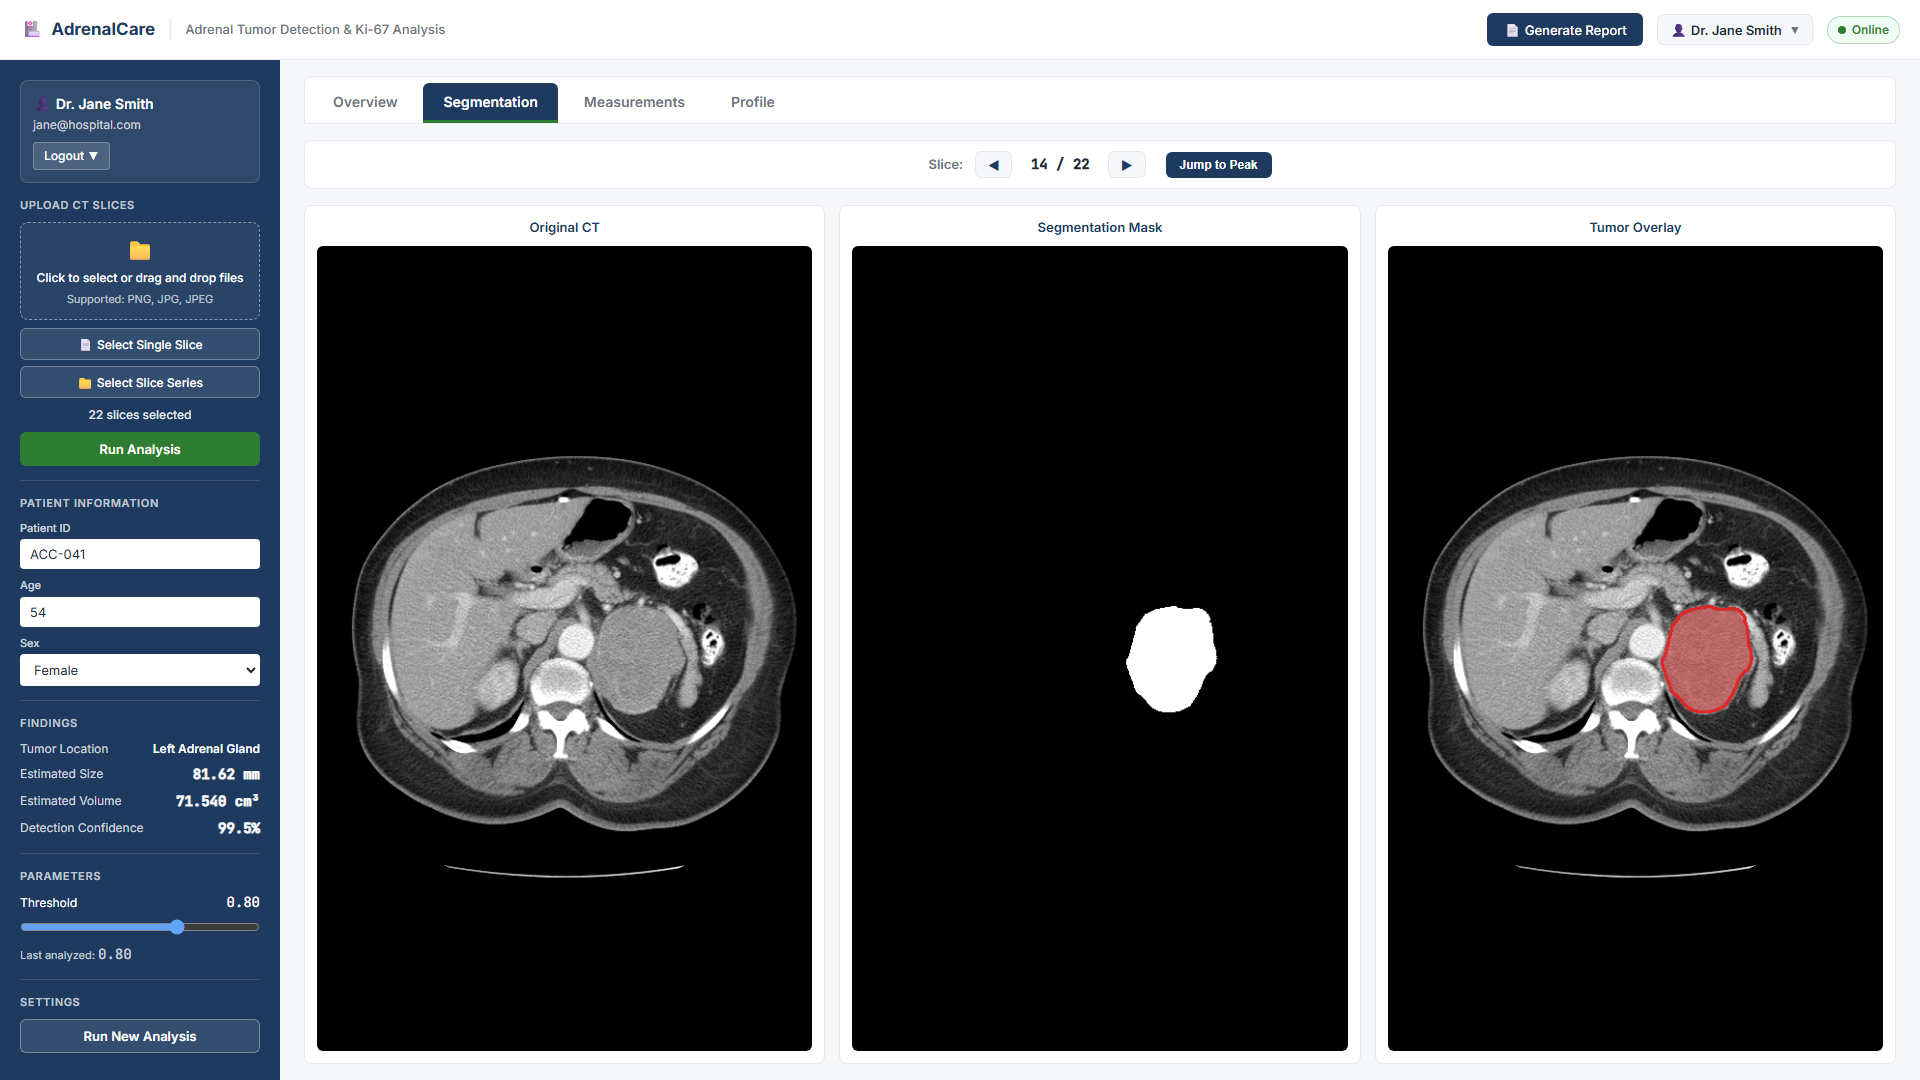
\includegraphics[width=0.98\columnwidth]{figures/fig_segmentation.png}
\caption{Segmentation interface displaying raw axial CT (left), predicted binary mask (center), and red boundary overlay (right) for patient slice series.}
\label{fig:segmentation}
\end{figure}

\begin{figure}[!t]
\centering
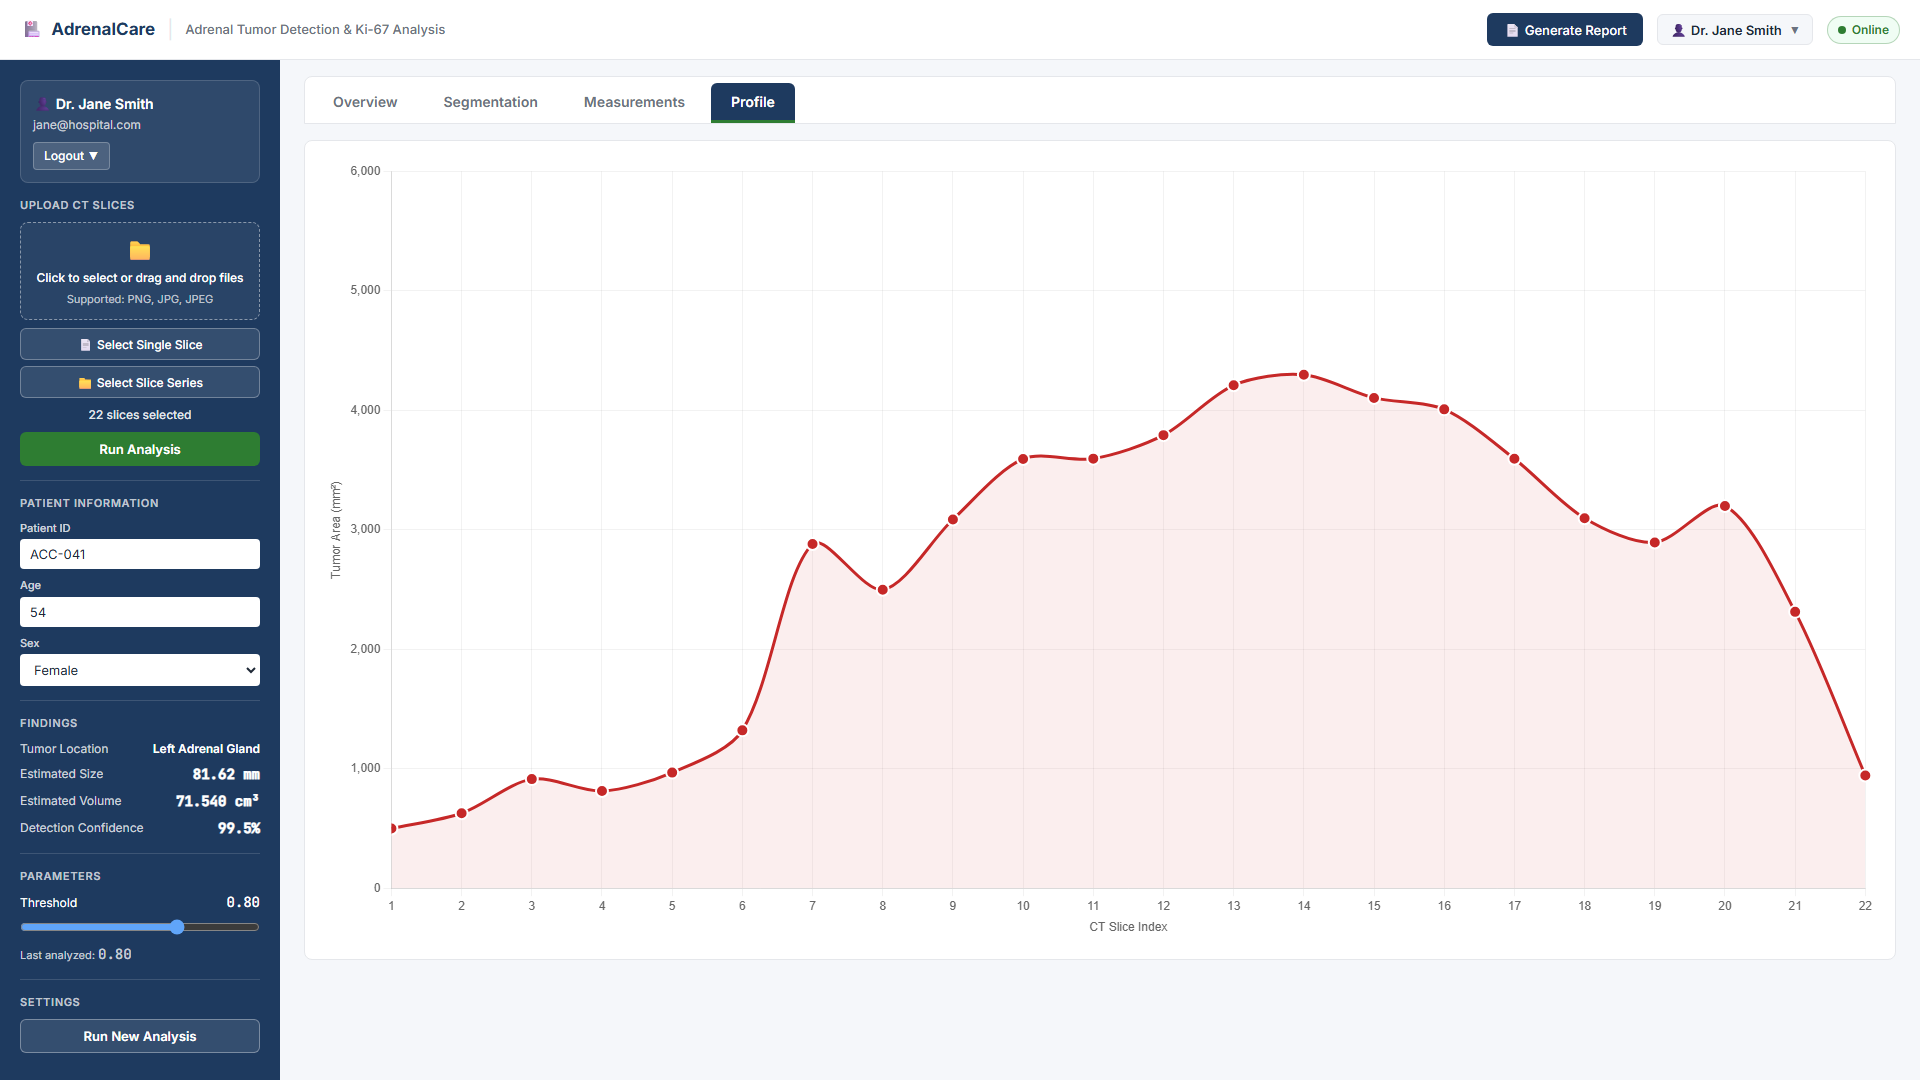
\includegraphics[width=0.98\columnwidth]{figures/fig_profile.png}
\caption{Continuous craniocaudal tumor area distribution ($mm^2$) plotted across CT slice series, showing the peak cross-sectional burden slice.}
\label{fig:profile}
\end{figure}

\section{Experimental Results and Discussion}

\subsection{Image-Level Detection Evaluation}
System performance was evaluated on the 295 unseen test slices (255 ground-truth positive, 40 ground-truth negative). Applying the detection threshold $\tau = 0.80$ produced the confusion matrix: $\text{True Positive (TP)} = 236$, $\text{False Positive (FP)} = 28$, $\text{True Negative (TN)} = 12$, and $\text{False Negative (FN)} = 19$.

\begin{table}[htbp]
\caption{Image-Level Detection Performance (Test Cohort, $N = 295$)}
\begin{center}
\begin{tabular}{llr}
\toprule
\textbf{Metric} & \textbf{Mathematical Definition} & \textbf{Value} \\
\midrule
Sensitivity (Recall) & $\text{TP} / (\text{TP} + \text{FN})$ & 92.55\% \\
Precision (PPV) & $\text{TP} / (\text{TP} + \text{FP})$ & 89.39\% \\
F1-Score & $2 \cdot \frac{\text{Precision} \cdot \text{Recall}}{\text{Precision} + \text{Recall}}$ & 90.94\% \\
Overall Accuracy & $(\text{TP} + \text{TN}) / \text{Total}$ & 84.07\% \\
Specificity (TNR) & $\text{TN} / (\text{TN} + \text{FP})$ & 30.00\% \\
\bottomrule
\end{tabular}
\end{center}
\label{tab:detection}
\end{table}

The 92.55\% sensitivity satisfies oncologic screening requirements by limiting missed tumor slices to 6.4\%. The lower specificity (30.00\%) stems from boundary slices where the upper pole of the kidney or splenic margins produced mild edge responses, which the post-processing component size filter largely suppresses.

\subsection{Pixel-Level Segmentation Overlap}
\begin{table}[htbp]
\caption{Segmentation Overlap Accuracy on Held-Out Test Set}
\begin{center}
\begin{tabular}{lrr}
\toprule
\textbf{Evaluation Metric} & \textbf{All Test Slices} & \textbf{Tumor Slices Only} \\
\midrule
Mean Dice Similarity & 53.60\% & 57.31\% \\
Mean Intersection over Union & 47.93\% & 50.74\% \\
Pixel Classification Accuracy & 99.05\% & 98.42\% \\
Peak Single-Slice Dice Score & --- & 95.94\% \\
\bottomrule
\end{tabular}
\end{center}
\label{tab:segmentation}
\end{table}

Representative individual slices showed high boundary alignment with ground truth:
\begin{itemize}
    \item Patient 015, Slice 114: $\text{Dice} = 0.9594, \text{IoU} = 0.9219$
    \item Patient 002, Slice 031: $\text{Dice} = 0.9184, \text{IoU} = 0.8491$
    \item Patient 008, Slice 134: $\text{Dice} = 0.8935, \text{IoU} = 0.8076$
    \item Patient 015, Slice 089: $\text{Dice} = 0.8332, \text{IoU} = 0.7141$
\end{itemize}

\subsection{Volumetric Robustness Across 53 Patients}
Across all 53 cohort volumes, estimated tumor masses ranged from 26.59\,cm$^3$ in early localized disease (Patient 014) to 7,863.83\,cm$^3$ in advanced invasive presentations (Patient 040). The model successfully processed this range without numerical divergence or failure on large retroperitoneal masses.

\subsection{Clinical Dashboard Deployment}
The pipeline is hosted via a responsive Flask application. Clinicians can drag and drop single slices or complete directories. The user interface features an interactive 3-panel viewer (Fig.~\ref{fig:segmentation}), an automated craniocaudal tumor burden curve (Fig.~\ref{fig:profile}), calibrated physical dimension displays, and a clean print stylesheet for PDF diagnostic report export.

\section{Limitations and Future Scope}
The model operates on 2D axial slices rather than full 3D volumetric convolutions, limiting inter-slice spatial context. Future iterations will evaluate 3D nnU-Net backbones \cite{isensee2021} and multi-organ networks \cite{gibson2018} to differentiate benign adrenal adenomas from malignant carcinomas. Linking CT radiomic signatures directly with microscopic Ki-67 proliferative indices remains an active direction.

\section{Conclusion}
This study presented an automated deep learning pipeline for Adrenocortical Carcinoma detection, segmentation, and morphometric analysis in axial CT series. Trained on the TCIA benchmark with patient-level stratification, the U-Net architecture achieved 92.55\% detection recall, 89.39\% precision, and 90.94\% F1-score on held-out test data, with a peak segmentation Dice coefficient of 95.94\%. Automated calculation of cross-sectional area, 3D volume, and spatial tumor burden curves, integrated into an accessible clinical dashboard, provides surgical teams with rapid, objective anatomical measurements to support preoperative planning.

\section*{Acknowledgment}
The authors thank the Department of Computer Science and Engineering at Maharaja Institute of Technology Thandavapura (MIT Thandavapura) for institutional support. We also acknowledge the contributors of the TCIA Adrenal-ACC-Ki67-Seg dataset at MD Anderson Cancer Center for providing annotated medical imaging data.

\begin{thebibliography}{10}
\bibitem{moawad2023}
A.~W. Moawad, A.~A. Ahmed, M.~ElMohr, et~al., ``Voxel-level segmentation of pathologically-proven Adrenocortical carcinoma with Ki-67 expression (Adrenal-ACC-Ki67-Seg),'' \emph{The Cancer Imaging Archive (TCIA)}, 2023. DOI: 10.7937/1FPG-VM46.

\bibitem{fassnacht2018}
M.~Fassnacht, O.~M. Dekkers, T.~Else, et~al., ``European Society of Endocrinology Clinical Practice Guidelines on the management of adrenocortical carcinoma in adults,'' \emph{European Journal of Endocrinology}, vol. 179, no.~4, pp. G1--G46, 2018.

\bibitem{ronneberger2015}
O.~Ronneberger, P.~Fischer, and T.~Brox, ``U-Net: Convolutional networks for biomedical image segmentation,'' in \emph{Proc. MICCAI}, LNCS, vol. 9351, pp. 234--241, 2015.

\bibitem{clark2013}
K.~Clark, B.~Vendt, K.~Smith, et~al., ``The Cancer Imaging Archive (TCIA): Maintaining and operating a public information repository,'' \emph{Journal of Digital Imaging}, vol. 26, no.~6, pp. 1045--1057, 2013.

\bibitem{heller2021}
N.~Heller, F.~Isensee, K.~H. Maier-Hein, et~al., ``The state of the art in kidney and kidney tumor segmentation in contrast-enhanced CT imaging: Results of the KiTS19 challenge,'' \emph{Medical Image Analysis}, vol.~67, p. 101821, 2021.

\bibitem{isensee2021}
F.~Isensee, P.~F. Jaeger, S.~A. Kohl, et~al., ``nnU-Net: a self-configuring method for deep learning-based biomedical image segmentation,'' \emph{Nature Methods}, vol.~18, no.~2, pp. 203--211, 2021.

\bibitem{bilic2023}
P.~Bilic, P.~Christ, H.~B. Li, et~al., ``The Liver Tumor Segmentation Benchmark (LiTS),'' \emph{Medical Image Analysis}, vol.~84, p. 102680, 2023.

\bibitem{litjens2017}
G.~Litjens, T.~Kooi, B.~E. Bejnordi, et~al., ``A survey on deep learning in medical image analysis,'' \emph{Medical Image Analysis}, vol.~42, pp. 60--88, 2017.

\bibitem{wang2021}
S.~J. Wang, E.~B. Habra, and K.~Elsayes, ``Imaging of Adrenocortical Carcinoma: Current concepts and practice,'' \emph{American Journal of Roentgenology}, vol. 216, no.~5, pp. 1200--1210, 2021.

\bibitem{gibson2018}
E.~Gibson, F.~Giganti, Y.~Hu, et~al., ``Automatic multi-organ segmentation on abdominal CT with dense networks,'' \emph{IEEE Trans. Med. Imaging}, vol.~37, no.~8, pp. 1822--1834, 2018.
\end{thebibliography}

\end{document}
